\documentclass{article}


\usepackage[utf8]{inputenc}
\usepackage[justification=centering]{caption}
\usepackage{multicol}
\usepackage{todonotes}
\usepackage[super]{nth}

\captionsetup{justification=raggedright,singlelinecheck=false}


\title{Machine Learning Enabled Mouse-Brain Segmentation}
\author{
 Hendrik Klug \\
  Master Student\\
  Department of Electrical Engineering\\
  ETHZ\\
  \texttt{klugh@student.ethz.ch} \\\date{January 2020}}

\begin{document}


\maketitle

\begin{abstract}
%%briefly explain why
%%  - extraction ROI 
%%  - registration into a standard reference space
As part of the analysis of high-field mouse MRI data, relevant brain tissue needs to be selected via a mask.
For this process to be performed automatically, brain voxels need to be classified based both on their signal intensity and position in the image.
Nowadays, deep neural networks are the state-of-the-art methods for tissue segmentation in biomedical imaging, and thus constitute a promising method for preclinical neuroscience.
%% outperforms current methods is a pretty high bar. We haven't really compared it to e.g. BET and other heuristic human-MRI-derived classifiers. You can still make the case that it is better, but that's a case you need to make on theoretical grounds unless you have data for the comparison.
We present a deep learning enabled framework for segmentation of brain tissue in functional and structural MR images, \textit{that outperforms \textbf{current methods}, requiring only a fraction of the processing time needed by them}.
\end{abstract}
%\newpage

%\begin{multicols}{2}

\section{Background}
In order to make meaningful comparisons across subjects inside a study, it is imperative that the images lie in a standard reference frame.
Because of positioning imprecision and anatomical animal variations, this is not the case for the original MR acquired images.
To solve this issue, the images need to be projected into the reference frame via registration. 
Intensities outside the brain region of a mouse MR image present high variations and bias the registration process.
As a remedy, it would be useful to extract the region of interest and perform the registration on it.
For this purpose, we propose a machine learning enabled brain extraction in an additional node to the workflow presented by Ioanas et al. \cite{ioanas_optimized_2019}.
The additional node creates a mask of the brain region with segmentation using a classifier and masks the image such that only the region of interest remains.
\todo{registration on masked image is much better: show results}


\subsection{Convolutional Neural Networks} \label{sec:Convolutional Neural Networks}
In recent years it has been shown that convolutional neural network give the best results for semantic image segmentation in terms of precision and flexibility \cite{geng_survey_2018} \cite{ronneberger_u-net:_2015}.
Training a convolutional neural network into a classifier is a supervised method, meaning that the model needs to learn its parameters based on observations of data.

The training data set of a classifier is as important as the architecture of the model itself.
To improve general-purpose application, training examples need to be drawn from a usually unknown probability distribution, that is expected to be representative of the space of occurrences.
We define the space of occurrences as the space of which the data of interest is drawn from.
In our case this consists of all the different mouse brain MRI data sets coming from multiple experiments, with their corresponding labels. 
Ideally experiment setups are uniform and the resulting data does not differ much, but small variations in the experiment setup and animal size are unavoidable.
Based on an approximation of the occurrence space, the network has to build a general model that enables it to extrapolate and produce sufficiently accurate predictions in new cases.
Manually creating annotations as required to train a deep-learning classifier for high-resolution data is often infeasible, as it requires manual expert segmentation of vast amounts of slices.

While our purpose was to create a workflow that generates better masks than the ones used for registration\todo{this is wrong, cite where the mask comes from}, we showed that the latter could be used as training data for the deep-learning model, by applying small changes to them.

\section{The Classifier}
\subsection{Model}
As the architecture of the classifier, the U-Net from Ronneberger et al \cite{ronneberger_u-net:_2015} was chosen based on its high performance in the field of biomedical image segmentation.
This is a convolutional neural network that consists of a contracting path that captures context in addition to a symmetric expanding path that enables precise localisation.
Localisation in this context means that a class label is assigned to each pixel.
We used the U-Net implementation from zhixuhao \cite{zhixuhao_zhixuhao/unet_2020}, written in Keras.
Keras is a high-level neural networks API, written in Python and capable of running on top of TensorFlow, CNTK, or Theano.
It allows for a easily readable code and makes it thus easier to reproduce.

The implementation of the U-Net from zhixuhao has two drop-out layers in addition to the original one.
A drop-out layer randomly sets a fraction of input units from the layer to 0 at each update during training time.
The set fraction rate is 0.5.
It is known that dropout helps prevent overfitting and greatly improves the performance of deep learning models \cite{srivastava_dropout:_nodate}.

Three losses were tested for the training of the model, namely the Dice-loss, the binary-cross-entropy loss and the sum of both.

The Dice-loss is computed from the Dice score. It calculates the similarity of two binary samples X and Y with
$$D_{coef} = \frac{2|X\cap Y|}{|X|+|Y|}$$
It is a quantity ranging from 0 to 1 that is to be maximised.
The loss is then calculated with $1-D_{coef}$.
Because the Dice loss is not differentiable, small changes need to be made.
In our case, the two samples to be compared are normalised, grey valued images  and are thus not binary but have values between 0 and 1. 
Additionally, instead of using the logical operation \textit{and}, element wise products are used to approximate the non-differentiable intersection operation.
To avoid a division by zero, $+1$ is added on the numerator and denominator.

Because many more pixels in the masks are 0 than 1, there is a class imbalance problem.
It is a problem, because in this case a false positive gives a much higher loss than a false negative.
For example, predicting only black would give an acceptable loss, while predicting only white pixels would not.
Using the Dice coefficient as a loss function for training should make it invariant to this class imbalance problem as stated by Fausto Milletari et al. in \cite{milletari_v-net:_2016}.

The binary cross-entropy loss, also called Log loss, is defined by:
$$H_p (q) = -\frac{1}{N} \sum ^N _{i=1} y_i \cdot log(p(y_i))+(1-y_i) \cdot log(1-p(y_i))$$
For pixel values of 0 and 1, it adds $log(p(y))$ for each white pixel (y=1) and $log(1-p(y))$ for every black pixel (y=0) to the loss.

We quickly realised that the Dice-loss gives the best results for our problem and therefore used it to train the model. \todo{compare results}

\subsection{Training}
The model was trained slice wise, with the coronal view and 600 as the maximum number of epochs.
The coronal view was chosen over the axial one, because the shapes of the masks are much simpler in the coronal view and thus easier to learn for the network.
Additionally the coronal view has the advantage of higher resolution as the MR images were recorded coronally.

To improve the learning process of the network, two callbacks from Keras were used \cite{noauthor_callbacks_nodate}. "ReduceLROnPlateau" reduces the learning rate when the validation loss has stopped improving and "EarlyStopping" stops the training when the validation loss has stopped improving for a number of epochs.
The latter reduces computation time and prevents overfitting.

\subsection{Data Set}
The data set consists of 3D MR images taken from an aggregation of three studies; irsabi , opfvta \cite{ioanas_whole-brain_nodate}, drlfom \cite{ioanas_effects_nodate} and other unpublished data, acquired with similar parameters. \todo{cite} 

The images are transformed into a standard space with one defined mask via SAMRI \cite{noauthor_ibt-fmi/samri_2019} and are thus defined in the same affine space.
SAMRI is a data analysis package of the ETH/UZH Institute for Biomedical Engineering.
It is equipped with an optimized registration workflow and standard geometric space for small animal brain imaging \cite{ioanas_optimized_2019}.

Because of variance in mouse brain anatomy and in the experiment setup, some of the transformed data do not overlap perfectly with the reference template.
To filter these images out, most of the incongruent slices were removed manually from the data set.

For the registration of the images, a padding was needed to make the originally not affine space affine. 
Due to this, the 3D volumes present many zero-valued slices, some of them overlapping with the mask.\todo{show example}
\begin{figure}
    \centering
    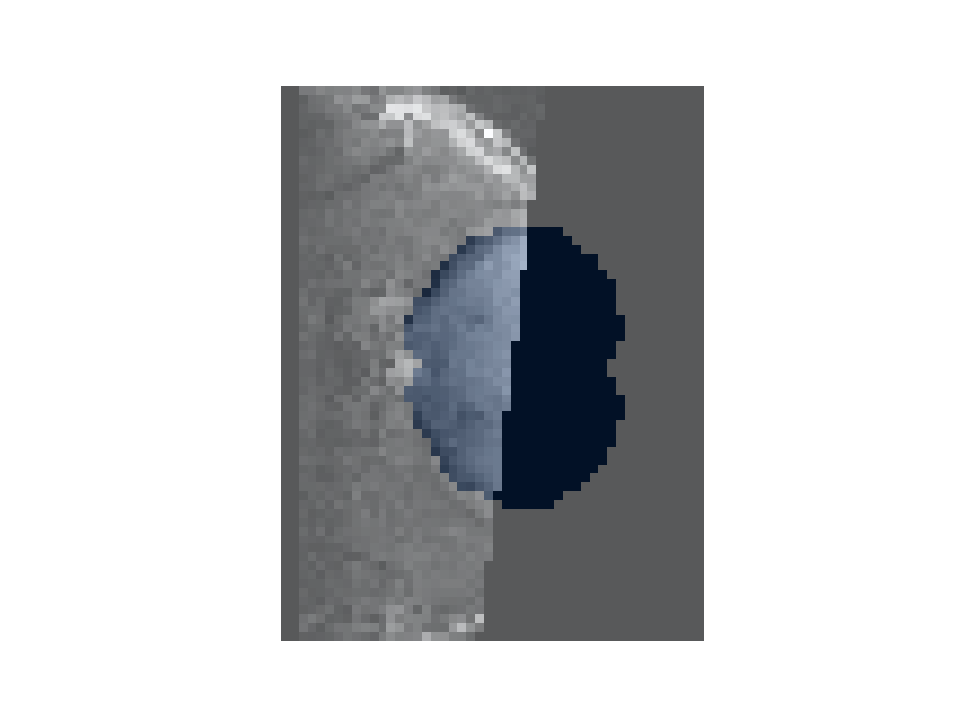
\includegraphics[width = 0.5 \textwidth]{mask_not_overlap.pdf}
    \caption{Caption}
    \label{fig:my_label}
\end{figure}
Since it is not wanted for the model to predict a mask on black slices, the mask is set to zero where the image is as well.
Because some pixels representing the brain tissue are zero-valued, holes result from this operation.
To patch these, the function binary\_fill\_holes from scipy.ndimage.morphology \cite{noauthor_multi-dimensional_nodate} is used.

In the coronal view, each slice of the transformed data is originally of shape (63, 48), matching the reference space resolution of \SI{200}{\micro\metre}.
It is then reshaped into (64, 64) by adding a zero padding to the border.

Finally, the images are normalised by first clipping them from the minimum to the \nth{99} percentile of the data in order to remove outliers and then divided by the maximum.

\subsection{Data Augmentation}

Because of diverse settings in the experiment setup, including animal manipulations causing artifacts, MR image quality can differ substantially between labs and even individual study populations.
To account for these variations, we apply an extensive set of transformations to our data.
This includes rotations of up to 90$^{\circ}$, a width and height shift range of 30 pixels, a shear range of 5 pixels, zoom range of 0.2 and horizontal as well as vertical flips.

This not only increases the data set size but also makes it more representative of the general data distribution of Mice brain MR images and results in a model with a better generalisation capability.

Many more sophisticated methods have been tested, but it has been shown that one of the more successful data augmentation strategies is the simple transformations mentioned above \cite{perez_effectiveness_2017}.

\section{Methods}
The slice-wise predictions of the model are reconstructed to a 3D mask via the command \textit{Nifit1Image} from the neuro-imaging python package nibabel \cite{noauthor_neuroimaging_nodate}.
This is done using the same affine space as the input image.









\section{Results}

\section{Conclusion}


\bibliographystyle{unsrt}
\bibliography{references}
%\end{multicols}
\end{document}
